\section{Background}
\subsection{Problem Context}
This problem's main focus is the difficulty of organising classical sheet music, and how this can be made easier by the automatic extraction of key pieces  of information. In order to understand what a performer may want to know about a particular piece, it is important to have a brief understanding of the elements of musical notation common to all compositions.

The key element of this form of notation is the staff, as shown in figure \ref{fig:staff}. This is a grouping of five horizontal lines, with each line or space in the staff indicating a different sound pitch, a term meaning the relative "highness" or "lowness" of the sound \parencite{classroom}.

\begin{figure}[h]
    \centering
        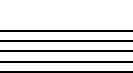
\includegraphics{staff-crop.pdf}
    \caption{A blank staff}
    \label{fig:staff}
\end{figure}

This staff is divided by bar lines, vertical lines delineating grouped units of sound and silence (formally referred to as notes and rests), which provides an indication of the unit's relationship in time by its juxtaposition to other groupings in the composition. These groupings are called measures or bars, with each bar having a variable maximum of notes and rests. 

\begin{figure}[h]
    \centering
        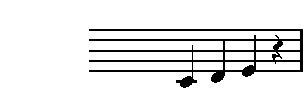
\includegraphics{bar_with_notes-crop.pdf}
    \caption{A bar containing three notes and one rest}
    \label{fig:staff-notes}
\end{figure}
\subsubsection{Clefs}
In the system of staff notation, sound frequencies, or pitches, are denoted by letters A-G - after each cycle of the letter names, the next pitch above it will be the start of a new cycle. The cycles are often split by octaves, a term meaning eight pitches, for example A to A or E to E. 

In order to provide a link between the lines and spaces of a staff and pitch name, a clef symbol is necessary.
\begin{figure}[h]
    \centering
        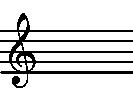
\includegraphics{clef-crop.pdf}
    \caption{A staff with a treble clef}
    \label{fig:clef}
\end{figure}

Each clef symbol denotes a different pitch name - figure \ref{fig:clef} shows a G. The center around which this symbol is drawn - in figure \ref{fig:clef}, the second line from the bottom of the staff - indicates that this line or space will be known as the pitch name denoted by the symbol. From this the reader can infer all other pitches by counting through the letters of the cyclic octave system, so in figure \ref{fig:clef}, the pitch above becomes an A, and the pitch below becomes an F.

This symbol is important to a musician as different clefs are used to position the majority of the pitches in a piece on the staff, as this makes it easier to read. From this a performer can infer the average range of a piece, and predict whether this will be comfortable for the performer's chosen instrument or voice.

\subsubsection{Keys}
A second important indication to the player is the key, denoted by a key signature.
\begin{figure}[h]
    \centering
        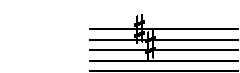
\includegraphics{key-crop.pdf}
    \caption{A staff with a key signature}
    \label{fig:key}
\end{figure}

A collection of symbols at the beginning of the piece indicate which pitches should be raised by half pitches, and which should be lowered. Raised pitches are called sharps, indicated by the \# symbol, whilst lowered pitches are called flats, indicated by the $\flat$ symbol. Each key, which has a letter name and key type (which can either be "major" or "minor"), has a different combination of flats or sharps. 

This is a useful piece of notation to a musician as pieces in less common keys, such as C\# major or F\# major, may prove more difficult for the user to perform, and therefore they may want to filter out pieces in these particular keys. Similarly, in the case of singers, a singer's range may sit comfortably in one or two keys and they would perhaps want to find pieces in only these keys. 

\subsubsection{Meter}
The third symbol denoted at the beginning of a measure is the meter or time signature, displayed as two numerals positioned like a mathematical fraction.

\begin{figure}[h]
    \centering
        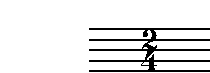
\includegraphics{meter-crop.pdf}
    \caption{A staff with a 2/4 time signature, or meter}
    \label{fig:meter}
\end{figure}

The upper number of a meter symbol indicates the amount of beats in the bar. A beat simply refers to a note or rest, and the type of beat is indicated by the lower number. In the case of figure \ref{fig:meter}, 2/4 indicates a measure will contain 2 crotchets, or quarter-length notes. The most common time signature is 4/4, which for this reason is usually denoted with a C in place of the fraction, meaning "Common time".

This information is important as it tells the performer how the rhythm and beat of the piece should be felt, counted and performed, and is useful for searching purposes as different meters give the piece a different feeling, dictating the sort of occasion this piece would accompany. 

For example, 2/4 is commonly used for march pieces, and 3/4 is commonly used for waltzes and dance pieces.

\subsubsection{Tempo}
The speed of a particular piece, or the tempo, is indicated by an equation.

\begin{figure}[h]
    \centering
        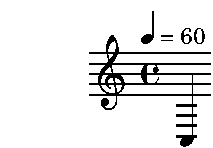
\includegraphics{tempo-crop.pdf}
    \caption{A staff with tempo marking}
    \label{fig:tempo}
\end{figure}

The equation above the staff in figure \ref{fig:tempo} indicates that the piece should be played at 60 beats per minute. The symbol dictating the sort of beat per minute depends on the time signature, here a crotchet (or quarter note) is given as the piece is in 4/4 time. Sometimes, this will be accompanied by a text direction to indicate speed or style, such as Andante, indicating a walking speed.

This indication would prove a useful identifier as pieces of different tempos provide variation in performance lists, so a concert organiser may want to find pieces with a variety of tempos.

\subsubsection{Further metadata}
Aside from these symbols, there are some items of textual information useful to the user. 

The first of these would be the parts in the piece and their transpositions. A part refers to a grouping of measures given to one performer, as shown in figure \ref{fig:parts}. "Part" used in a general sense usually refers to the names given to the left, in this example, "Clarinet in B$\flat$" and "Flute".
\begin{figure}[H]
\centering
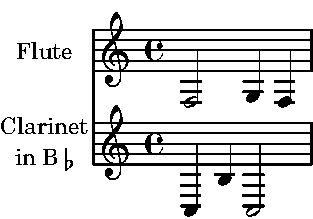
\includegraphics{multiparts-crop}
\caption{Two separate parts in one score}
\label{fig:parts}	
\end{figure}



Parts would be relevant as a particular group of instrumentalists may need parts that fit their instruments. If this is not the case for a given piece, however, a part written for a different instrument, for example, the Alto Saxophone rather than the Tenor Horn, may be compatible with the instrument anyway, if the transposition matches the instruments together. 

An instrument which has a transposition means that, whilst most instruments would play a note as it is written, a transposing instrument will automatically sound the note in a different key, as described earlier, which may raise or lower the sound of the instrument. For example, the note C played on an Alto Saxophone will sound as an E$\flat$, because it is in the key of E$\flat$ major. 

Further to this, the user would want to know the piece's title, and names of publishers, composers, arrangers and lyricists of the work, commonly known as the bibliography of a piece\parencite{MIR}. Further to the composer name, it may be useful to know the date of composition as an indication of the era in which the piece was composed, such as Classical/Baroque/Romantic, though this would not always be written on the sheet music so may need to be researched using the internet.

\subsubsection{Music Information Retrieval as a research area}
The area in which this project is set is called Music Information Retrieval, with the idea of this area being to provide users with more ways to find and identify written and audio music\parencite{MIR}. In particular, this project deals with what is termed by \cite{MIR} as the "Multi Faceted problem", as one piece of music may have many ways in which it can be defined - above are some key pieces of information which this project will use, but there are many more used by other projects.

Due to the multi faceted problem having many different layers and areas which different research projects have been interested in, there does not appear to be a standard meta model defined in research - this is because projects relating to the production of music by machines may require modelling of how tonal melodies are produced\parencite{creativeMachines}, whilst historical projects may need more information about bibliography, sound production projects may need more information about instruments being used and how to synthesise their outputs and countless other research areas will be interested in more complex piece information. This is described by \cite{MIR} as the multi disciplinary problem, and it is for this reason that the project has defined its own meta model described in the previous sections of the problem context, rather than reuse another model. It is hoped by open sourcing this project that the meta model contributions of this project will help later projects to define a standard model for future music information research projects.

\subsection{Comparison of Technologies}
\subsubsection{Programming Language}
This project could be developed with a variety of programming languages, as displayed in table \ref{table:langs}.

\begin{table}[H]
\centering
\begin{tabular}{| l | l | l | l |} \hline
  {Language} & {Speed of development} & {Developer's Knowledge} & {Most recent use} \\ \hline
  C\# & Fast & A lot & 2nd year \\ \hline
  Python & Fast & A lot & In constant use for over a year \\ \hline
  C++ & Slow & Average & 2nd year \\ \hline
\end{tabular}
\caption{Table of languages considered}
\label{table:langs}
\end{table}
The three key elements of whether a language is suitable for this project are speed of development, as the time constraint of a year means it is important that development is not hindered by the language itself, developer knowledge and most recent usage of the language as this will provide an additional time benefit. These are displayed in table \ref{table:langs}.

A further consideration is platform independence, as the developer intends to make the project accessible to all users. It is understood that C\# is platform independent through the use of the Mono Project, which is feature-complete to C\# 10 \parencite{MonoDev}, or Xamarin Studio and other such tools, but the developer has not developed any applications with C\# for use on multiple operating systems. For this reason, the developer feels more comfortable using Python, owing to the experience of writing applications for Linux and Windows in previous projects. 

The developer has also considered the Open Source communities and repositories around each of the languages. Whilst not important in the context of the current project, after the project is completed it is intended that the project be Open Sourced to contribute to further research in this area, and considering the graph in figure \ref{fig:graph} \parencite{Redmonk}, Python has the highest percentage of repositories on the popular Open Source repository website Github of the three languages considered. Whilst this does not categorically prove it as the best language for Open Source software development, it shows that there are a high number of users and projects in this area, which will make it a more popular project to work with once open sourced.

\begin{figure}[h]
\centering
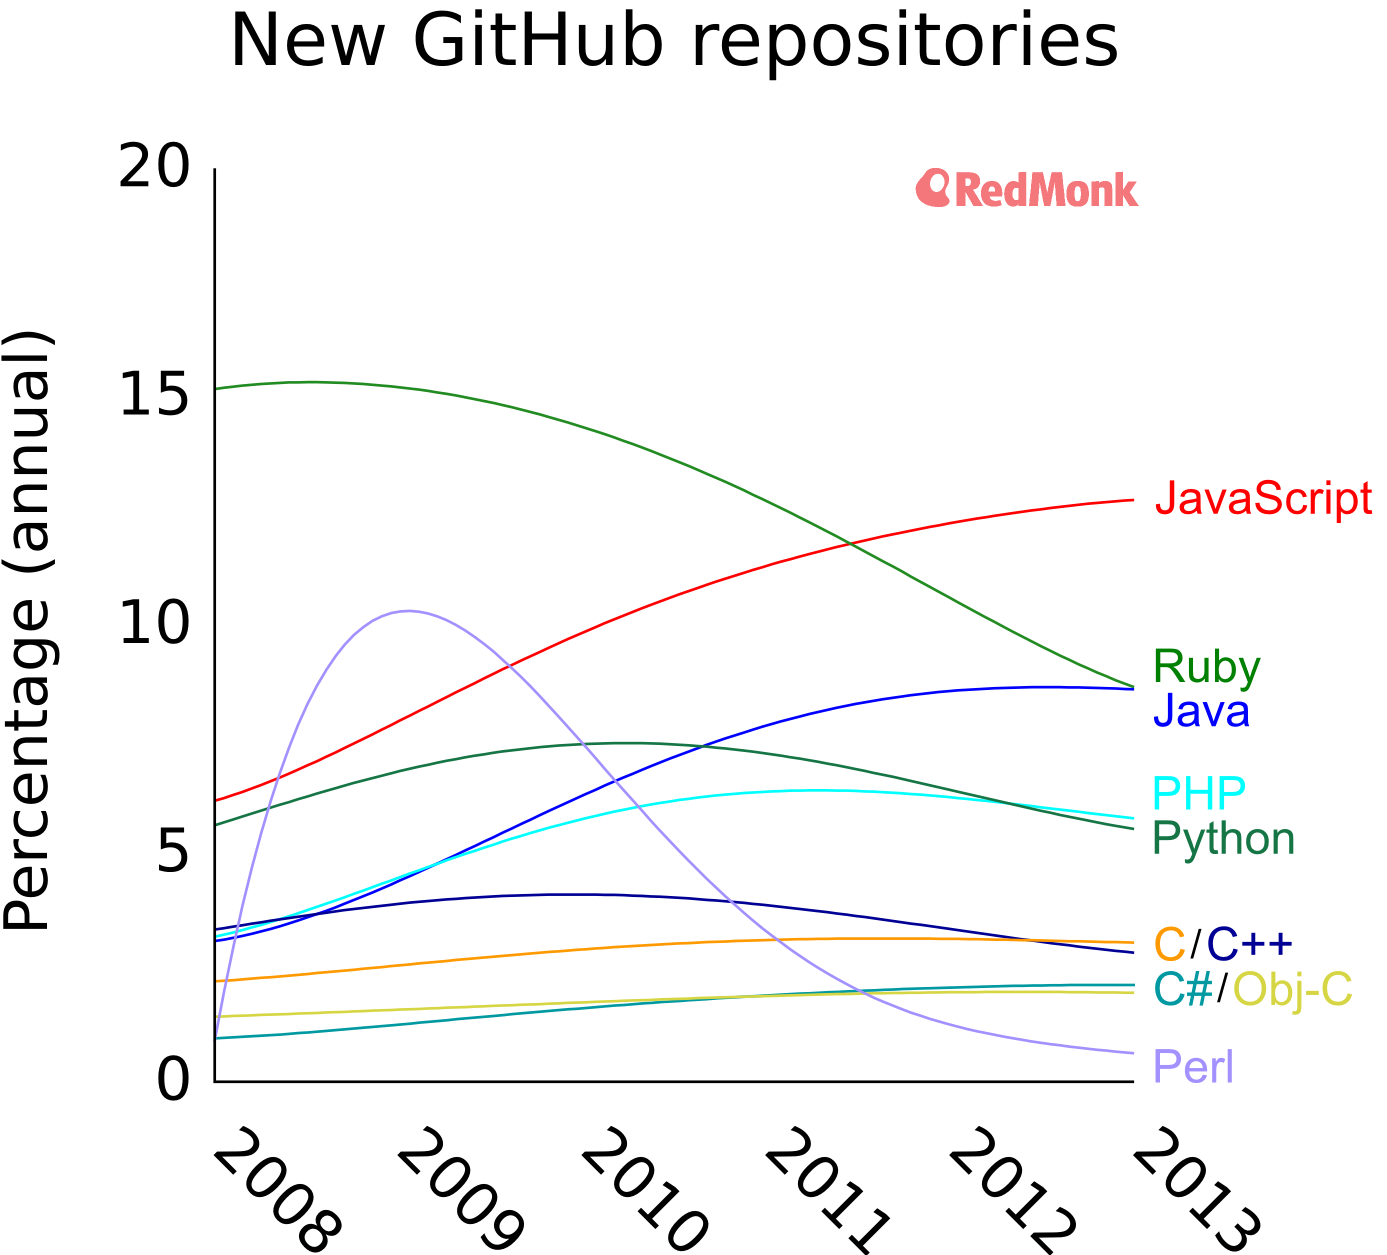
\includegraphics[width=250pt]{github-repos}
\caption{A graph showing the percentage of repositories on Github in different languages}	
\label{fig:graph}
\end{figure}

Furthermore, there are many projects in the field of musical software research currently in existence using this language, \parencite{pmus} such as mingus, an advanced music theory and notation package for Python.

It is for these reasons that Python has been chosen as the development language. Beyond the selection of Python, it is important to discuss and consider which version to use, as Python 3 was introduced in 2008, but Python 2 continues to be maintained and was updated to include many of the backwards compatible features in 2010. Whilst this seems an obvious choice as Python 3 is the latest version, many projects still have issues updating and using Python 3 as it was deliberately not backwards compatible \parencite{Foundation2}.

Upon due consideration, Python 3 has been selected, though if the project requires legacy libraries this may have to be evaluated again. This decision has been made because at this stage the project does not appear to require libraries which do not work with Python 3, and therefore the developer should make every effort to keep the project up to date with the latest version.

\subsubsection{File format}
The project will require at least one default format for it to process music, which needs to have detailed information about what the score contains. Table \ref{table:formats} describes the options considered.

\begin{table}[H]
\centering
\begin{tabular}{| c | c | } \hline
  {Format} & {Purpose} \\ \hline
  muscx & MuseScore notation \\ \hline
  SIB & Sibelius notation \\ \hline
  new format & this project only \\ \hline
  MusicXML & sharing music between software \\ \hline
\end{tabular}
\caption{A table showing the different file formats considered}
\label{table:formats}
\end{table}
The first two options, muscx and SIB files, are formats used by the open source notation software MuseScore \parencite{MuseTour}, and the world's most popular proprietary notation software, Sibelius \parencite{avid}. Using either or both of these files would mean the majority of users would be able to use the application. 
However, both options couple this project with those particular packages, when users could still choose other software to write music with. Furthermore, the formats are specifically designed for those software packages and may have nuances which make development for this project more difficult. Additionally, Sibelius is proprietary so borrowing their file format may cause copyright issues.

The third option is to create an entirely new format. This would mean the file format was designed to the requirements of the project and therefore be entirely customisable and extensible. However, this project is created with the intention of organising, not composing music, so the project would also need to produce a converter from other file formats which is not desirable.

The fourth and final option is MusicXML, a file format intended for sharing and archiving the world's sheet music \parencite{mxml}. This particular format is used by a wide variety of software packages \parencite{mxml} and is included in the formats usable by both MuseScore \parencite{MuseTour} and Sibelius \parencite{avid}, therefore neither couples the format with a program nor requires manual creation and import of current music files. 

However, this particular format was designed by a third party, Make Music, who have a vested interest in the file format and it's structure as they produce Finale, another popular music editing package\parencite{mxmlSoft} and might therefore present a further technical challenge in learning how the format notates everything, and may not reflect the same design intentions as this project.

For reason of inclusion in composition software packages, MusicXML has been selected as the file format for the project. This adds an advantage to the project over the composition software packages mentioned as the project will be designed to work well with MusicXML, whilst those mentioned are designed to work with their own file formats and thus have some issues converting to MusicXML\parencite{mscoreBugTracker}, meaning that this project will be more precise in it's rendering of MusicXML.

\subsection{Comparison of Algorithms for Rendering Music}
Figure \ref{fig:flow} shows a flow diagram for the system of rendering sheet music. Each decision taken in order to reach this method will be discussed in detail below.
\begin{figure}[H]
    \centering
    \includegraphics[width=80pt]{render_algorithm-crop}
    \caption{A flow diagram describing the rendering system}
    \label{fig:flow}
\end{figure}

\subsubsection{Algorithms for parsing XML to memory}
For the rendering of sheet music, the system must in some way manipulate an XML file to an output format.

The first option for this would be applying an XSL stylesheet, which is commonly the method of choice for rendering XML files in a web browser. This is not an option in MusicXML because the notation is too complicated and requires too many symbols, whilst XSL stylesheets are usually used for images and text representations. Sheet music is somewhere in between the two, and thus this option cannot be selected.

The second option would be to create or reuse a converter script from XML to the output format, meaning the output would be generated at the same time as the input. However, this couples the system with MusicXML and would slow down development if it were required to use a different additional input, or decisions were made to change the output format. Furthermore, the Big O representation of this type of script to any output format is $O(n^2)$, whilst the selected final option using objects would be $O(n)$.

The final option, which has been chosen for the project, is to create a converter script which would parse the MusicXML and create a hierarchy of objects. This avoids coupling directly to MusicXML as new formats of both input and output would only need a converter script creating to the object hierarchy which would then handle input or output to other formats.

However, whilst this avoids coupling, a technical challenge is created using this method in that the object structure needs careful planning to cater for the structure of MusicXML and the structure or method of output, which with little knowledge of the input or output format is difficult to achieve.

\subsubsection{Rendering Algorithm}
The program is required to take the object structure and transform it, in some way, to musician readable sheet music. The user should be able to pan around the sheet music and zoom in and out of it to view specific details.

This could be achieved using an entirely new algorithm, with the output going directly to the render window using different glyphs and fonts extracted from their relevant classes.

However, the functionality of panning and zooming using this algorithm may be difficult to optimise, as both could possibly require running the algorithm each time the user provides input. 

Furthermore, the conversion of even basic sheet music to a readable format would require a high level of precision and complexity, and creating a new algorithm would be considered reinventing the wheel, so to speak, as this is a process that has been covered by many different applications (like MuseScore \parencite{MuseTour}, Finale \parencite{mxml} and Sibelius \parencite{avid}). 
Lastly, the process of debugging whether the symbols are correct would require visual checking and would be difficult to debug automatically.

It would be possible to alleviate the panning and zooming problem by converting the collection of symbols to an image or PDF file and using a built in image rendering library, such as wxPython \parencite{WX}. However, this method still involves reinventing the wheel and incurs problems with visual debugging.

Considering these factors, it has been decided that the algorithm will be outputting files to a third party system known as Lilypond. Lilypond is a language and system developed to typeset the highest quality sheet music \parencite{Lilypond}, which takes an input file and outputs a PDF or image. As this is a language unto itself and has been in development for many years by the Open Source community, this will alleviate the problem of visual debugging - instead, each class can create a formatted Lilypond output based on its attributes and unit tests can automatically confirm that the result is as expected.

This adds a further technical challenge as the design aims of MusicXML as explained in an earlier section were found to be very different from the design aims of Lilypond. Designing the system and structure around both objects at the start of the project was difficult, due to the developer's lack of knowledge of both formats and frameworks, and thus changes were made late into the project that set back development time.

Furthermore, as rendering of sheet music is not the main aim of this project, it was decided that specific areas of notation should not be included in order to ensure that other areas of the project, such as metadata extraction, did not have a significantly shorter development time, and to ensure that all implemented objectives were implemented to a high quality, at the expense of rendering all symbols. In most areas, the information is not lost completely as it is imported from the MusicXML file into the object structure, but ignored upon request for render of a given piece.

\subsubsection{Algorithms for parsing XML for information}
For the parsing of XML itself, there are two potential built in methods to choose from. The first, known as DOM or Document Object Model, loads the entire XML file into memory and provides methods to search the loaded file for specified tags. The developer has used this before in personal and industrial projects, and believes it is cumbersome to manipulate data in this way. Furthermore, this project is focussing on rendering the information rather than rendering it with precise formatting, and many software packages implant musicXML files with very complex formatting information which may or may not be necessary\parencite{MusicXMLPresentation}.

The second option is using a different api called the Simple API for XML (SAX). In this method, the program loads the XML file tag by tag, and connects to call backs when specified things occur in the file, for example a new tag or piece of data inside tags, or the closing of an old tag. This is easier to work with as functionality can iteratively be built up by creating handlers for each tag, and is better for memory management as only tags which are necessary to the project will have any effect on the object structure. For these reasons, this method has been selected.

\subsubsection{XML verification algorithm}
For both the algorithm options discussed in section 3.3.1, a further choice is whether to verify the XML parsed, using an online file validator, or presume the file is written in valid MusicXML. 

The usual choice is to verify all XML, and is therefore the default option for both methods of parsing. Whilst this confirms that XML is valid before starting parsing of a file which could be corrupt, the speed at which files will parse is greatly reduced according to the speed of the user's internet connection.
Furthermore, if the user is browsing their own music collection, it should not be necessary for the user to be connected to the internet.

Due to speed and functionality considerations, the choice has been made that the XML parser algorithm will not verify XML being converted to objects, or being examined for metadata. Given that most musicXML will be produced automatically by other programs, it is unlikely files opened by the project will be corrupt, though necessary steps will be taken to avoid this causing a problem in the program.

\subsection{Comparison of Algorithms for Organising Sheet Music}
The system design for the automatic extraction of meta information for each sheet music file is described by the flow diagram in figure \ref{fig:meta}. 
\begin{figure}[H]
    \centering
    \includegraphics[width=250pt]{metadata_algorithm-crop}
    \caption{A flow diagram describing the meta scanning system}
    \label{fig:meta}
\end{figure}

Figure \ref{fig:uiLoader} shows how the user interface will load the information and apply the rendering algorithm. Finally, figure \ref{fig:metaSearching} shows how search and autocomplete will function. The decisions made in order to arrive at these methods shall be discussed and compared in the following subsections.
\begin{figure}[H]
    \centering
    \includegraphics[width=250pt]{UI_loading_algorithm-crop}
    \caption{A flow diagram describing the loading of metadata and usage in the User Interface}
    \label{fig:uiLoader}
\end{figure}
\begin{figure}[H]
    \centering
    \includegraphics[width=250pt]{search_algorithm-crop}
    \caption{A flow diagram describing the loading of metadata and usage in the User Interface}
    \label{fig:metaSearching}
\end{figure}

\subsubsection{Metadata Scanning algorithm}
The metadata algorithm has been designed so that, for a given folder, the program will parse all of the files with the XML extension for a given selection of information (for example, composer, piece title, instruments - the full details of the meta model are described in the problem context). Based on development and testing of this algorithm, the data will be cached to a permanent file in order to ensure unchanged files do not have to be parsed more than once.

It would be possible to store this data in memory using a generic type or a record object. This would be easy to implement and designed to the requirements of the system, but would be reinventing the wheel as SQL was developed for this purpose\parencite{SQLite}.

It has therefore been decided that the algorithm will store all data to an SQLite file using several tables to link the data together, and not create an in memory object. This will be much faster than using a developer defined object as database systems store data using a B-Tree and have been optimised to be faster than any sorting algorithm that could be produced during the course of this project\parencite{SQLiteBTree}.

This also means that the system does not need to create a cache file and means that the future improvements or developments will not have to use python to access the data, as SQLite has built in APIs in most programming languages.

\subsubsection{XML data acquisition algorithm}
The system should take in a selection of XML files and parse them for information. As described previously, this could use either the DOM method of XML parsing, or the SAX method of parsing.
The system will use SAX because there are only a select few tags and collections of information that the database will need to peruse, and SAX means that only these tags will have an effect on the algorithm or memory.

\subsubsection{Metadata Searching Algorithm}
The application should allow the user to input a search query and find results which match the input. A user can then select from a list of result options which will render the selected file.

It has been decided that the input will allow for both simple strings, such as 4/4 or quarter=half when defining time signatures and tempos, and for more complex input, such as instrument:clarinet with:clef:alto. This will enable users to search without needing to know or use too much search syntax and is aimed to be intuitive and simple.

The alternative would be to allow only key value pairs or define a new search syntax which the user would need to learn. However, as this application is being developed for musicians who may not have the patience or desire to learn a querying language, the decision has been taken to make the search syntax as intuitive as possible.

\subsection{Comparison of Technologies for Importing Online Musical Sources}
\subsubsection{Musical Sources}
Two open and free sources of sheet music have been selected for potential inclusion, which will enable users to increase their own music collections with new music without using a browser to peruse collections. The first is \textbf{MuseScore Online}, which is a community website created for composers to upload, share and discover compositions using the MuseScore platform \parencite{MuseShare}.

This has been selected due to the number of files available, the openness of the platform and the well documented API. It will, however, be necessary to manage copyright issues, as pieces published on this website may be published under the license of the composer's choosing and therefore may cause issues with certain types of users, in particular those performing commercially.

The second selected source is the \textbf{IMSLP}. This is the \textbf{International Music Score Library Project}, built with the intention of sharing the world’s public domain music, and contains 290,000 scores to date \parencite{imslp}. This may be a questionable source, as not all pieces are uploaded in MusicXML format due to the pieces being scanned and uploaded by community members, rather than being automatically generated by a piece of software. However, this source does not raise any copyright issues as all pieces are no longer covered by copyright.

It may also be possible to import collections from subscription services and websites enabling purchase of music, such as \textbf{MusicNotes.com}. However, this will require closer contact with the companies maintaining the website and may not be appropriate for an educational and academic purpose.

\subsubsection{Searching Algorithm}
The APIs for both selected sources provide a variety of output formats, the 2 most prominent being XML and JSON. The algorithm for browsing the source from the program will need to in some way, contact the server to confirm whether there are pieces which have a specific attribute entered by the user, and download the file if the piece is selected.

It would be possible to use an algorithm which repeatedly connects to the API and polls for the relevant input from the user, returning a list of options which the user would then select from and download from the server. Whilst this would be simple to implement, this would make the program considerably slower, as it would require repeated connection to the internet. This would also cause problems for the maintainers of the server, as repeated requests from a piece of software would cause a heavy load on the server.

If possible, the software should cache a copy of all metadata served from each online source to alleviate this problem, and search for the relevant inputted data from this, and then, if necessary, collect the relevant file from the server. This would require a connection to the server only twice - once when updating metadata sources, and once when downloading a file - rather than a persistent or repeated connection. 

However, this needs confirmation from the sources selected that caching is an accepted API algorithm, as some websites stipulate that this is not allowed, and therefore the present decision is to use the previous option until this has been confirmed.

\subsection{Comparison of Algorithms for Sound Output and Image Input}
\subsubsection{MIDI algorithm}
The sound output algorithm must, for a given part or selection of parts, output the sheet music to a MIDI or MP3 file, which can then be played within the program. 

It has been decided that each class in the solution will have a method to produce this output, in the same way as the algorithm described for rendering in section 3.3.4, which will be combined into an output file and played.

This creates an extendible architecture, as it would easily be possible to create output methods to other formats in the future.

\subsubsection{Image input algorithm}
In order to import images or flat files into the chosen file format, it will be necessary for the program to include the ability to apply music optical character recognition to the file, and save the output to MusicXML, which can then be parsed by other parts of the program. 

It would be possible for a new algorithm to be produced for converting new imported images into the chosen file format. This would mean the algorithm  could be optimised according to the project aims, and provide sufficient technical challenge.

However, this project is concerned with music organisation, not optical music recognition specifically, and as such the project is too large to commit a sufficient amount of time to this particular algorithm in order to make it function as well as other algorithms. 

As a reference point, Optical Character Recognition for natural languages has taken many years to develop and perfect, and has been an attractive research area and idea to a wide variety of users \parencite{InternationalConf}. OMR, or Optical Music Recognition, has been the focus of international research for over three decades, and while numerous achievements have been made, there are still many challenges to be faced before it reaches its full potential \parencite{musicocr}. 

It has therefore been decided that OCR as a topic is too large for this project, and if this goal is included in the project, it will be through communication with other systems, such as Audiveris, an open music scanner \parencite{audiveris}. 

This removes the technical challenge of producing an entirely new algorithm, but adds the challenge of understanding how optical music recognition scanners work, and how they can be integrated with the system, particularly if the third party package is not developed in Python.

\subsection{Alternative Solutions}
Table \ref{table:software} shows the alternative options considered in the area of Sheet Music organisation automation. This shows that the closest alternative would be Power Music Pro, though much of the functionality changes slightly according to the platform it has been developed for \parencite{PowerMusic}. Furthermore, Power Music Pro's only improvement on manual organisation is the ability to search by lyric, whilst this project intends to allow for a cross section of other organisation techniques, as explained in the problem context.

Additionally, each of the possible options are released in a commercial environment, with Avid's Photoscore being too expensive for the average user.  Seemingly, this project would constitute the only free and Open Source software released for this problem.

A final point to make is that none of these solutions provide a version for Linux based operating systems, whilst this project should be useable on Mac, PC and Linux based operating systems.
\begin{table}[H]
\centering
\begin{tabu} to 1.05\textwidth {| X[l] | X[c] | X[c] | X[c] | X[c] | X[c] | X[c] | X[c] | X[c] |} \hline
{Software} & {Rendering of Sheet Music} & {Manual Organisation} & {Automatic Organisation by complex notation} & {Connection to Online Sources} & {Audio Playback} & {OMR} & {Price} & {Platform} \\ \hline
Avid Scorch & \checkmark & \checkmark & $\times$ & \checkmark & \checkmark & $\times$ & £1.40 \parencite{AvidScorch} & iOS \\ \hline
Power Music Pro/Power Music Mac & \checkmark & \checkmark & partial & \checkmark & \checkmark & $\times$ & £49 for PC, £29 for Mac \parencite{PowerMusic} & PC \& Mac  \\ \hline
Avid Photoscore & \checkmark & $\times$ & $\times$ & $\times$ & $\times$ & \checkmark & £200 \parencite{Pscore} & PC \& Mac \\ \hline
Scorcerer & \checkmark & \checkmark & $\times$ & $\times$ & \checkmark & \checkmark & £15 for iPad version, £26 for Mac and PC \parencite{Scorcerer} & iPad, Mac \& PC \\ \hline
\end{tabu}
\caption{A comparison table of other available software}
\label{table:software}	
\end{table}
